\documentclass[dvisvgm,tikz,border=4pt]{standalone}
\usepackage{amsmath,amssymb}

\usetikzlibrary{arrows.meta,positioning,automata,shapes,shapes.misc,calc,decorations.pathmorphing,decorations.markings,angles,quotes,patterns,mindmap,matrix,knots,hobby,trees}
\tikzset{->-/.style={decoration={markings, mark=at position 0.5 with {\arrow{Stealth}}}, postaction={decorate}}}
\begin{document}
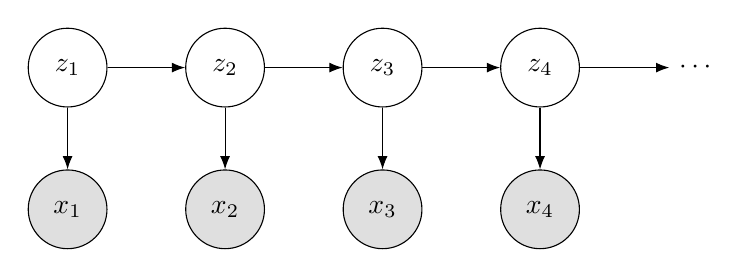
\begin{tikzpicture}[s/.style={circle, draw, minimum size=10mm}, o/.style={s, fill=gray!25}, >=Latex]
\foreach \i in {1,...,4} {
  \node[s] (z\i) at (2*\i,0) {$z_\i$};
  \node[o] (x\i) at (2*\i,-1.8) {$x_\i$};
  \draw[->] (z\i) -- (x\i);
}
\foreach \i [count=\j from 2] in {1,...,3} \draw[->] (z\i) -- (z\j);
\node (dots) at (10,0) {$\cdots$}; \draw[->] (z4) -- (dots);
\end{tikzpicture}
\end{document}
